% Chapter 1

\chapter{Introduction} % Main chapter title

\label{Intorduction} % For referencing the chapter elsewhere, use \ref{Chapter1} 


%----------------------------------------------------------------------------------------

\section{Motivation}
This report is an exploration of the intersection of two broad movements and the possibilities of social and technology system \cite{Sociotechnology} convergence through the specific application of blockchain technology to facilitate governance in cooperative organisations. The first "movement", comprises technical developers offering possible technical solutions to a range of social, economic, political and environmental challenges. These tech solutions currently fall within the emergent notion of Web 3.0. The second "movement", is a diverse socio-economic and political one concerned with shaping the emergent relationships between individuals and authorities, in a world recently interconnected by the internet. Both the technological and social developers in these areas are essentially focused on the rights of the individual, the terms on which they participate in social, economic, political and environmental domains.\\

\begin{figure}
\centering
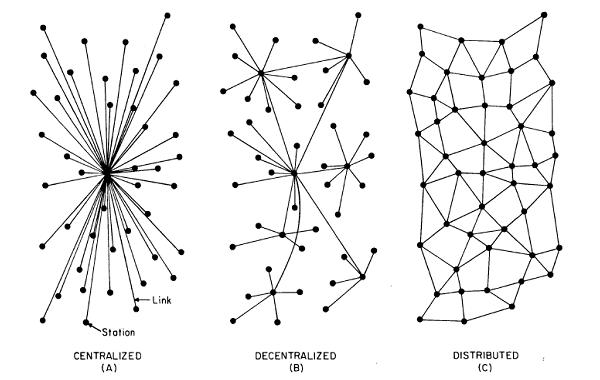
\includegraphics[width=\textwidth]{Figures/baran_net}
\decoRule
\caption[networks]{Centralized, Decentralized and Distributed Systems (Paul Baran, 1964)}
\label{fig:Electron}
\end{figure}

In 2014, on the 25th birthday of the World Wide Web, Tim Berners Lee listed his six goals for the future of the web:  re-decentralisation, openness, inclusion, privacy, free expression and security \cite{berners_lee}.  Despite enabling the hyper acceleration of that most fundamental of human activities: communication and, therefore, the speed at which we are now able to exchange not only information, but also values, the web has yet to fulfil the potential envisaged by it's creator.  The desire for openness, privacy, inclusion and free expression are typical concerns for the 'netizens' of today. \\

Over the past fifteen years, we have witnessed the explosion and monopolisation of web services and digital technology. The critical role of the web in modern society means that a handful of corporations now have alarming levels of political and economic power. \\

Netizens have sacrificed privacy for convenience and quality for control.\\

In this context, Snowden's revelations \cite{Snowden}, which implicate most of the 'internet giants' \cite{nsa_giants} (NSA's PRISM \cite{Prism} program and work with GCHQ to undermine encryption systems\cite{nsa_undermine}), has magnified growing tensions between the rights of citizens on the one hand and the "needs" of governments and corporations to control on the other. Distrust and dissatisfaction has pushed many developers and critics to propose alternative ways of constructing and organising the web, ways that are promoted as being truer to the dream of Tim Berners Lee. 

\subsection{Technical Solutions}
The trend for decentralised solutions, popularly referred to as Web 3.0, within the tech community can be observed from the emergence of new organisations (for example, redecentralize.org\cite{Redecentralise}, webwewant.org\cite{Webwewant}), new applications and services (for example, Firechat\cite{Firechat}, arkOS\cite{Arkos}, Solid\cite{Solid}, Mailpile\cite{Mailpile}) and even new hardware (for example, OPI\cite{OPI}, FreedomBox\cite{Freedombox}).\\

The most notable indicator however, is the recent rejuvenation of peer to peer systems. In the pure sense of the term\cite{p2pdef}, peer to peer networks are distributed systems by definition. The arrival of Bitcoin\cite{nakamoto2008bitcoin} dramatically increased the potential of peer to peer systems by introducing blockchains or distributed ledger technology (DLT). Blockchain networks allow peers to maintain a consistent view of shared data without the requirement for centralised authority. They are secure, transparent and far more resilient to attack and corruption than centralised alternatives.\\ 

The term Bitcoin 2.0 is now being used to describe a proliferation of new blockchain projects. One of the more established of these is Ethereum\cite{Ethereum}, a platform for building arbitrary applications on a blockchain.\\ 

In addition to blockchain networks, there are now also a number of peer to peer distributed file systems including IPFS (Inter Planetary File system \cite{Ipfs}), Maidsafe\cite{Maidsafe} and Storj\cite{Storj}. \\

The combination of blockchain platforms, distributed filesystems and other decentralised technologies is providing a framework for new forms of distributed web applications with significantly improved levels of availability, user control, security and privacy. \\

Designed in this way, services are also much more resilient to accidental, purposeful or environmental damage to the network (Consider the Google service dropout in 2013 resulting in 40\% drop of Internet traffic \cite{Google_outage}) and retrieving popular content, which is dynamically replicated across the network, is faster rather than slower. Efficient usage of bandwidth is particularly important given the increasing consumption of large data content (HD video etc), the networking of everything (Internet of Things, IoT) and the 4 billion users yet to come online\cite{Coming_online}.\\

Despite all the advantages a distributed web might bring, the tech community face a serious challenge of adoption. The 'internet giants' have established significant barriers to entry through the quality of their service offering. Providing a distributed alternatives it is understood will require a large amount of capital investment (ref Gupta?). \\

\subsection{Social Developments}
Characterising and describing current socio-economic "movements" attempting to imagine and build new social relationships in any detail is beyond the scope of this report. Broadly speaking, these movements (including, for example, P2P Foundation, opendemocracy, lasindias, community land trusts, "new economics") seem to be concerned with locating decision making close to those affected (distributed, decentralised), increasing participation and fairness (inclusivity), cooperation, transparency (openness) and sustainability. At the micro economic scale a number of business models have historically posed an alternative organisational alternative to the shareholder based private limited company, for example, worker and member cooperatives, Friendly or mutual benefit societies, trusts and more recently social enterprises and community interest companies. This report is focused on blockchain applications for cooperative enterprises. \\

Thus far the cooperative movement has failed to establish itself as a counterforce to narratives dominating the web and our new digital age that focus on brilliant ideas brought to market by Venture Capital. However, according to Michel Bauwens, of the P2P Foundation "cooperative enterprises are in the midst of a revival", that is "part of an ebb and flow of cooperativism, that is strongly linked to the ebb and flow of the mainstream capitalist economy."\cite{Open_cooperativism} \\

Included in this resurgence is the platform cooperativism initiative which promotes the restructuring of digital platforms as cooperative enterprises. In this spirit, issues of user control, privacy and security are tackled from a social perspective by reimagining the organisational forms of the 'centralised' service providers with a trusted, member controlled, inclusive alternative. \\

"The seeds are being planted for a new kind of online economy. For all the wonders the Internet brings us, it is dominated by an economics of monopoly, extraction, and surveillance. Ordinary users retain little control over their personal data, and the digital workplace is creeping into every corner of workers' lives." \cite{Platform_cooperativism}.\\


\subsection{Synthesis}
The founding proposition of cooperatives around the world is member participation in value creation and sharing. This applies equally at scale and whether the coop is "bricks and mortar" or an online platform.\\  

Fully engaging and mobilising members to participate has historically been problematic (see Myners\cite{Myners} for example) and raises serious questions about the best ways to create governance architecture that is fit for purpose. \\

One popular solution has been the creation of structures based around the election of "representatives" who mediate and aggregate individual member views to higher decision making levels. Historically, these governance architectures and their propensity to facilitate participation have been shaped by available information and communication technologies: the printed page and face to face social interactions. The resultant organisational structures have necessarily become hierarchical, not fully representative of the stakeholders, slow to execute decisions and open to the development of minority bias.\\

Digital information and communication technologies are changing the possibilities for social, economic and democratic participation and cooperation in all walks of life.\\

The first wave of Web 2.0 "social media" technologies have connected billions of people in new relationships. Facebook since 2003 has, for example, connected 1.5bn users. Many other applications (google drive, onedrive, icloud, yammer, slack, loomio etc) are built to enable "communities" to formally and informally cooperate and collaborate to create value and take decisions.\\

Web 3.0 or "re-distributed" web proposes concepts and tech that create new relationships between individuals, organisations and the data they create for mutual benefit. This is envisioned (see ref) as a shift from centralised to decentralised to distributed data.\\

The challenge for democratic member based economic or commercial enterprises is how to use these technologies and concepts to create competitive advantage using participative governance architectures that are trusted, secure, transparent, auditable, efficient and useable. \\

Conversely, the challenge for tech and digital communities is the harnessing of cooperative and solidarity organisational forms to develop quality web services that are able to compete with the incumbent offerings. \\

\section{Objectives}
Given the broad motivation, the objectives for this project have been threefold:
\begin{enumerate}
\item To investigate the Ethereum platform and surrounding technologies to develop insight into new forms of distributed web applications.
\item To develop an understanding of the state of the art and the practical and theoretical limitations of the technology.
\item To inform my investigation by developing a concrete application to address the governance challenges faced by new forms of global, distributed cooperative enterprises.
\end{enumerate}

\section{Contributions}
The contributions of the study are as follows:
\begin{itemize}
\item A first, proof of concept, Ethereum \& IPFS backed distributed application for co-operative governance called Go-op. Go-op allows co-operative members to establish and conduct governance on the Ethereum network. Co-operatives on Go-op can track membership, collect membership fees in Ether and table and vote on normal resolutions.
\item An in depth study into the emerging requirement for co-operative governance tools that can maintain member participation and representation at scale.
\item A detailed exploration and evaluation of the state of 'dapp' development using the Ethereum platform.
\end{itemize}


